% -*- latex -*-
%%%%%%%%%%%%%%%%%%%%%%%%%%%%%%%%%%%%%%%%%%%%%%%%%%%%%%%%%%%%%%%%
%%%%%%%%%%%%%%%%%%%%%%%%%%%%%%%%%%%%%%%%%%%%%%%%%%%%%%%%%%%%%%%%
%%%%
%%%% This text file is part of the source of 
%%%% `Introduction to High-Performance Scientific Computing'
%%%% by Victor Eijkhout, copyright 2012-9
%%%%
%%%% This book is distributed under a Creative Commons Attribution 3.0
%%%% Unported (CC BY 3.0) license and made possible by funding from
%%%% The Saylor Foundation \url{http://www.saylor.org}.
%%%%
%%%%
%%%%%%%%%%%%%%%%%%%%%%%%%%%%%%%%%%%%%%%%%%%%%%%%%%%%%%%%%%%%%%%%
%%%%%%%%%%%%%%%%%%%%%%%%%%%%%%%%%%%%%%%%%%%%%%%%%%%%%%%%%%%%%%%%


\acf{ML} is a collective name for a number of techniques that
approach problems we might consider `intelligent', such as image
recognition. In the abstract, such problems are mappings from a vector
space of \indexterm{feature}s, such as pixel values in an image, to
another vector space of outcomes. In the case of image recognition of
letters, this final space could be 26-dimensional, and a maximum value
in the second component would indicate that a `B' was recognized.

The essential characteristic of \ac{ML} techniques is that
this mapping is described by a --~usually large~-- number of internal
parameters, and that these parameters are gradually refined. The
learning aspect here is that refining the parameters happens by
comparing an input to both its predicted output based on current
parameters, and the intended output.

\Level 0 {Neural networks}

% https://www.youtube.com/watch?v=aircAruvnKk

The most popular form of \ac{ML} these days is \acf{DL}, or
\indextermdef{neural networks}. Let's start by explaining this term.

A neuron, in a living body, is a cell that `fires', that is, gives off
a voltage spike, if it receives certain inputs. In \ac{ML} we abstract
this to a \indextermdef{perceptron}: a~function that outputs a value
depending on certain inputs. To be specific, the output value is often
a linear function of the inputs, with the result
limited to the range~$(0,1)$.

If we write the inputs as a vector~$\bar x$, and we introduce a vector~$\bar w$
of \indextermdef{weights} of the same size, and a scalar \indextermdef{bias}~$b$;
and we have a function~$\sigma$ known as the
\indextermdef{sigmoid} that maps $\bbR\rightarrow(0,1)$, we write the
scalar output~$y$ as:
\[ \bbR\owns y = \sigma( \bar w^t\bar x+b ). \]
One choice for a sigmoid function is
\[ \sigma(z) = \frac{1}{1+e^{-z}}. \]
Since we typically have many perceptrons, we let $y$ be a vector.
Now we have weights and a bias for each component, so
\[ \bbR^n\owns \bar y = \sigma( W\bar x + \bar b ). \]

A few observations:
\begin{itemize}
\item
  As indicated above, the output vector typically has fewer components
  than the input, so the matrix is not square, in particular not
  invertible.
\item The sigmoid function makes the total mapping non-linear.
\item Neural nets typically have multiple layers, each of which is a
  mapping of the form $x\rightarrow y$ as above.
\end{itemize}

\Level 1 {Classification}

This output $y$ can be used as a numerical value,
or as classification through
\[ 
\begin{cases}
  x\in C &\hbox{if $y\geq 0$}\\
  x\not\in C&\hbox{if $y<0$}\\
\end{cases}
\]

\Level 0 {Learning the coefficients}

Now consider the problem of determining the coefficients of the neural
net: the $W$ matrix and the $\bar b$ vector. The key here is that we have
for an input $\bar x$ both the computed output $\bar y$ and the
`correct' output~$\tilde y$. With this we can compute the
\indextermbusdef{error}{function} (or \indextermbusdef{cost}{function})
$E=\|\bar y -\tilde y\|$, which is a complicated function of the
coefficients, and minimize this by setting the coefficients correctly.

Finding coefficients that give a zero error for one particular input
$\bar x$ is not hard, but they will likely give a bad error for
another input. (This is sometimes called \indexterm{over-fitting}.)
Therefore, learning typically involves cycling through a set of inputs
until the error is acceptable for all of them.

Given an input and true output $(x^t,r^t)$ and a computed output
of~$y^t$, we have a squared error of
\[ E = \frac12 (r^t-y^t)^2 = \frac12 \left[r^t- w^tx^t\right]^2. \]
Alternatively:
\[ E = \frac1n \sum_x E_x \]
where we have a set of $n$ samples~$x$.
This form of the error function allows us to compute partial
derivatives $\partial E/\partial w$ wrt some coefficient~$w$
for a single sample. We can then estimate the partial deriviate by
averaging over a number of samples.

We train the weights
by finding a (local) minimum, characterized by
\[ 0=\frac{d E}{d x} = \bigl( \frac{\partial E}{\partial x_j} \bigr)_j
    = \bigl( (r-y)x_j \bigr)_j \]
This can be done with \indexterm{gradient descent}:
\[ w\leftarrow w+\Delta w, \qquad b\leftarrow b+\Delta b\]
%%    \hbox{where $\Delta w=( \eta(r-y)x_j )_j$}. \]
where $\eta$ is a learning rate.
Per component this looks like:
\[ w_k \leftarrow w_k - \eta \frac{\partial E}{\partial w_k},
\qquad
b_k \leftarrow b_k - \eta \frac{\partial E}{\partial b_k},
\]

The linear function $y=w^tx$ is surprisingly useful. In fact, there is
a hard theoretical statement that says that enough of these functions,
followed by an appropriate normalization can approximate any
continuous function on a bounded domain.

\begin{quotation}
  \textsl{Universal Approximation Theorem}%
  \index{universal approximation theorem}

  Let $\varphi(\cdot)$ be a nonconstant,bounded, and
  monotonically-increasing continuous function. Let $I_m$ denote the
  $m$-dimensional unit hypercube $[0,1]^m$. The space
  of continuous functions on $I_m$ is denoted by
  $C(I_m)$. Then, given any function $f\in C(I_m)$
  and $\varepsilon>0$, there exists an integer
  $N$, real constants $v_i,b_i\in\mathbb{R}$ and
  real vectors $w_i \in \mathbb{R}^m$, where
  $i=1,\cdots,N$, such that we may define:
  \[
  F( x ) =
  \sum_{i=1}^{N} v_i \varphi \left( w_i^T x + b_i\right)
  \]
  as an approximate realization of the function $f$ where
  $f$ is independent of $\varphi$; that is,
  \[
  | F( x ) - f ( x ) | < \varepsilon
  \]
  for all $x\in I_m$. In other words, functions of the form
  $F(x)$ are dense in $C(I_m)$.
\end{quotation}

The function $y\leftarrow w^tx$ is called a \indextermdef{perceptron}.

\Level 1 {Backpropagation}

The process of `learning' consists of updating the weights and biases.
So let's take a single layer~$L$ with $y^{(L-1)}$ of the previous layer
as input, and output $y^{(L)}$ defined by
\[ y^{(L)} = \sigma\bigl( z^{(L)} \bigr),\qquad
z^{(L)}=W^{(L)}y^{(L-1)}+b^{(L)}. \]
The error function is
\[ E= \| y^{(L)}-\tilde y \|. \]
Then by the chain rule:
\[ \frac{dE}{dw^{(L)}} = \frac{dE}{dy^{(L)}}\cdot
\frac{dy^{(L)}}{dz^{(L)}}\cdot
\frac{dz^{(L)}}{dW^{(L)}} \]
where
\begin{itemize}
\item \[ \frac{dE}{dy^{(L)}} = 2(y^{(L)}-\tilde y) \],
\item \[ \frac{dy^{(L)}}{dz^{(L)}} = \sigma'(z^{(L)}) \],
\item \[ \frac{dz^{(L)}}{dW^{(L)}} = y^{(L-1)} \]
\end{itemize}

\Level 1 {Stochastic Gradient Descent}

In regression problems, we have a sample set $S\subset X$, and values
$f_x=f(x)$ for $x\in S$. The training problem is then to determine the
coefficients~$W=\{w_i\}_i$ that minimize the loss $\ell(x)=|F(x)-f_x|$,
or, with all parameters in place:
\[ \ell(x,W) = |F_W(x)-f_x| \]
The most popular algorithm for this is \acf{SGD}:
%
\begin{displayalgorithm}
  \While{not converged}
        { $x\leftarrow\hbox{random element from $S$}$\;
          $g\leftarrow\nabla \ell(x,W)$\;
          update $W$ with $g$\;
          }
\end{displayalgorithm}

\Level 1 {Linear discrimination}

A perceptron can be used to distinguish between two classes, by
looking at whether the output is positive or negative. This is
equivalent to using a `threshhold function' $s(\cdot)$ which takes
values 0,1 and looking at~$s(w^tx)$.

Often, the function~$s$ is taken as a sigmoid:
\[ \sigma(x) = \frac1{1+\exp{-w^tx}}. \]
(Note the appearance of such a function as~$\varphi$ in the approximation theorem
above.)

(Connection to posterior probability? Alpaydin~272)

\Level 0 {Multilayer networks}

Instead of a straightforward calculation $y\leftarrow w^tx$,
we can introduce a hidden layer as
\[ z_h = \sigma(w_h^tx) \]
and find the output~$y$ in terms of these hidden units:
\[ y_i = v_i^tz. \]

It is possible to introduce more than one hidden layer. This is often
a design decision, having a network that is `long and narrow' rather
than `short and fat'.

\Level 1 {Backpropagation}

\begin{figure}[ht]
  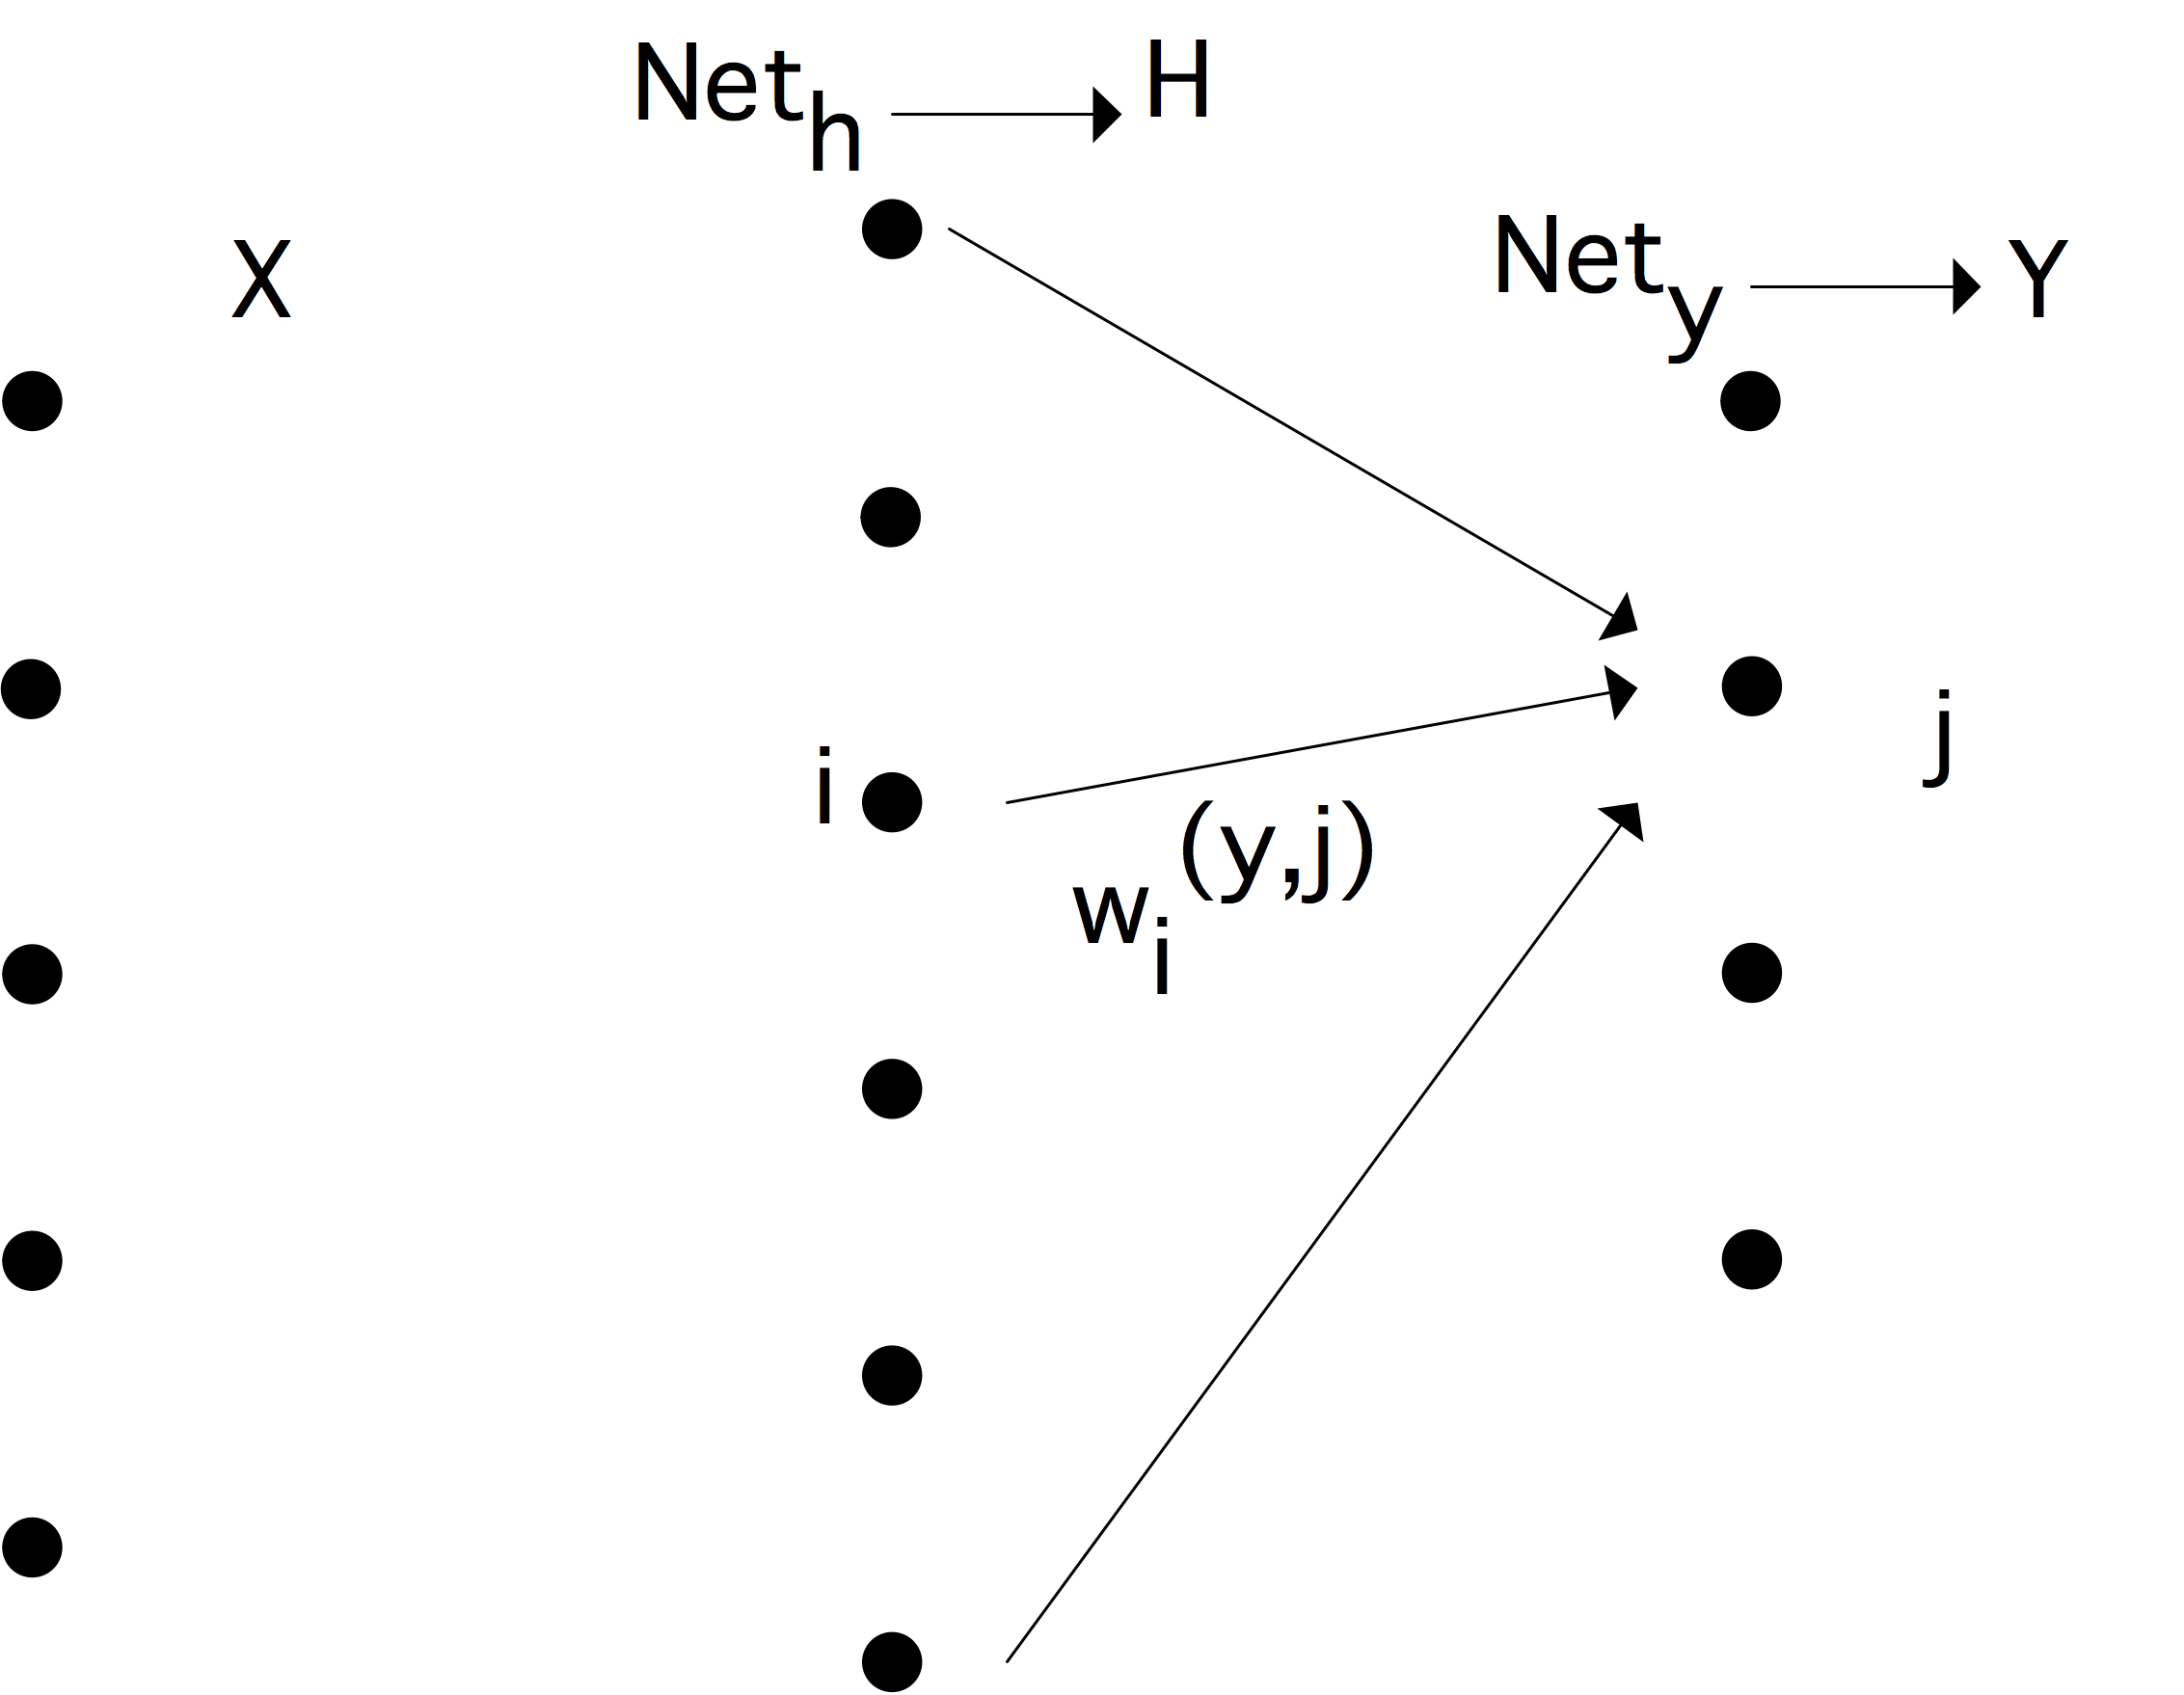
\includegraphics[scale=.12]{backpropagation-y}
  \caption{Back propagation, final layer coefficients}
  \label{fig:backprop-y}
\end{figure}

Let's describe a network with one hidden layer.
\def\net{\mathord{\mathit{Net}}}
\def\eE{{\cal E}}
\begin{itemize}
\item There is a set of inputs, $X$, of size~$n_x$.
\item On the intermediate layer,
  \[ \net^{(h)}= W^{ {(h)}^t }X \]
  where $W^{(h)}$ is a block of weight vectors:
  \[ \net^{(h)}_i = \sum_j w^{(h,i)}_jx_j. \]
\item The intermediate output values $H$ are formed with a sigmoid
  function:
  \[ h_i=\sigma\bigl(\net^{(h)}_i\bigr). \]
\item Net values on the output are computed from a second block of
  weights:
  \[ \net^{(y)}=W^{ {(y)}^t }H \]
  and we apply another sigmoid:
  \[ y_i=\sigma\bigl(\net^{(y)}_i\bigr). \]
\item We have a set of true output $T$ to compare against, and we
  measure the squared error
  \[ \eE=\frac12 E^tE,\qquad E=Y-T. \]
\end{itemize}

The problem is to compute the $W^{(h)}$ and $W^{(y)}$ coefficients to
minimize~$\eE$. We use some form of gradient descent.

The coefficients of the final layer are simple:
\begin{align}
  \frac{\partial\eE}{\partial w^{(y,j)}_i}
  &=E_j\frac{\partial y_j}{\partial w^{(y,j)}_i}
  &\hbox{$E_j$ is the only nonzero component}\\
  &=E_j \frac{\partial y_j}{\partial \net^{(y)}_j}
  \frac{\partial \net^{(y)}_j}{\partial w^{(y,j)}_i}
  &\hbox{chain rule}\\
  &=E_j y_j(1-y_j)
  \frac{\partial \net^{(y)}_j}{\partial w^{(y,j)}_i}
  &\hbox{use lemma~\ref{lemma:sigma-prime}}\\
  &=\delta_j h_i
  &\hbox{defining $\delta_j=E_jy_j(1-y_j)$}\\
\end{align}

In sum we get the update statement for the $j$-th colum of $W^{(y)}$
weights:
\[ W^{(y,j)} \leftarrow W^{(y,j)} - \epsilon \delta_j H \]
where $\epsilon$ is the learning rate.

For the intermediate layer coefficients we have to chain rule a couple
times more.

\begin{align}
  \frac{\partial\eE}{\partial w^{(h,j)_i}}
  &=\sum_{k=1}^{n_y} E_k\frac{\partial y_k}{\partial w^{(h,j)}_i}\\
  &=\sum_{k=1}^{n_y} \delta_k\frac{\partial \net^{(y)}_k}{\partial w^{(h,j)}_i}\\
  &=\sum_{k=1}^{n_y} \delta_k w^{(y,k)}_j
  \frac{\partial h_j}{\partial w^{(h,j)}_i}
  &\hbox{only $h_j$ contributes}\\
  &=\sum_{k=1}^{n_y} \delta_k w^{(y,k)}_j h_j(1-h_j)
  \frac{\partial \net^{(h)}_j}{\partial w^{(h,j)}_i}\\
  &=\sum_{k=1}^{n_y} \delta_k w^{(y,k)}_j h_j(1-h_j) x_i\\
\end{align}

We see that the final layer coefficients $W^{(y)}$ appear in this
formula for updating~$W^{(h)}$, which
is what gave this procedure the name \indextermdef{back propagation}.

\begin{figure}[ht]
  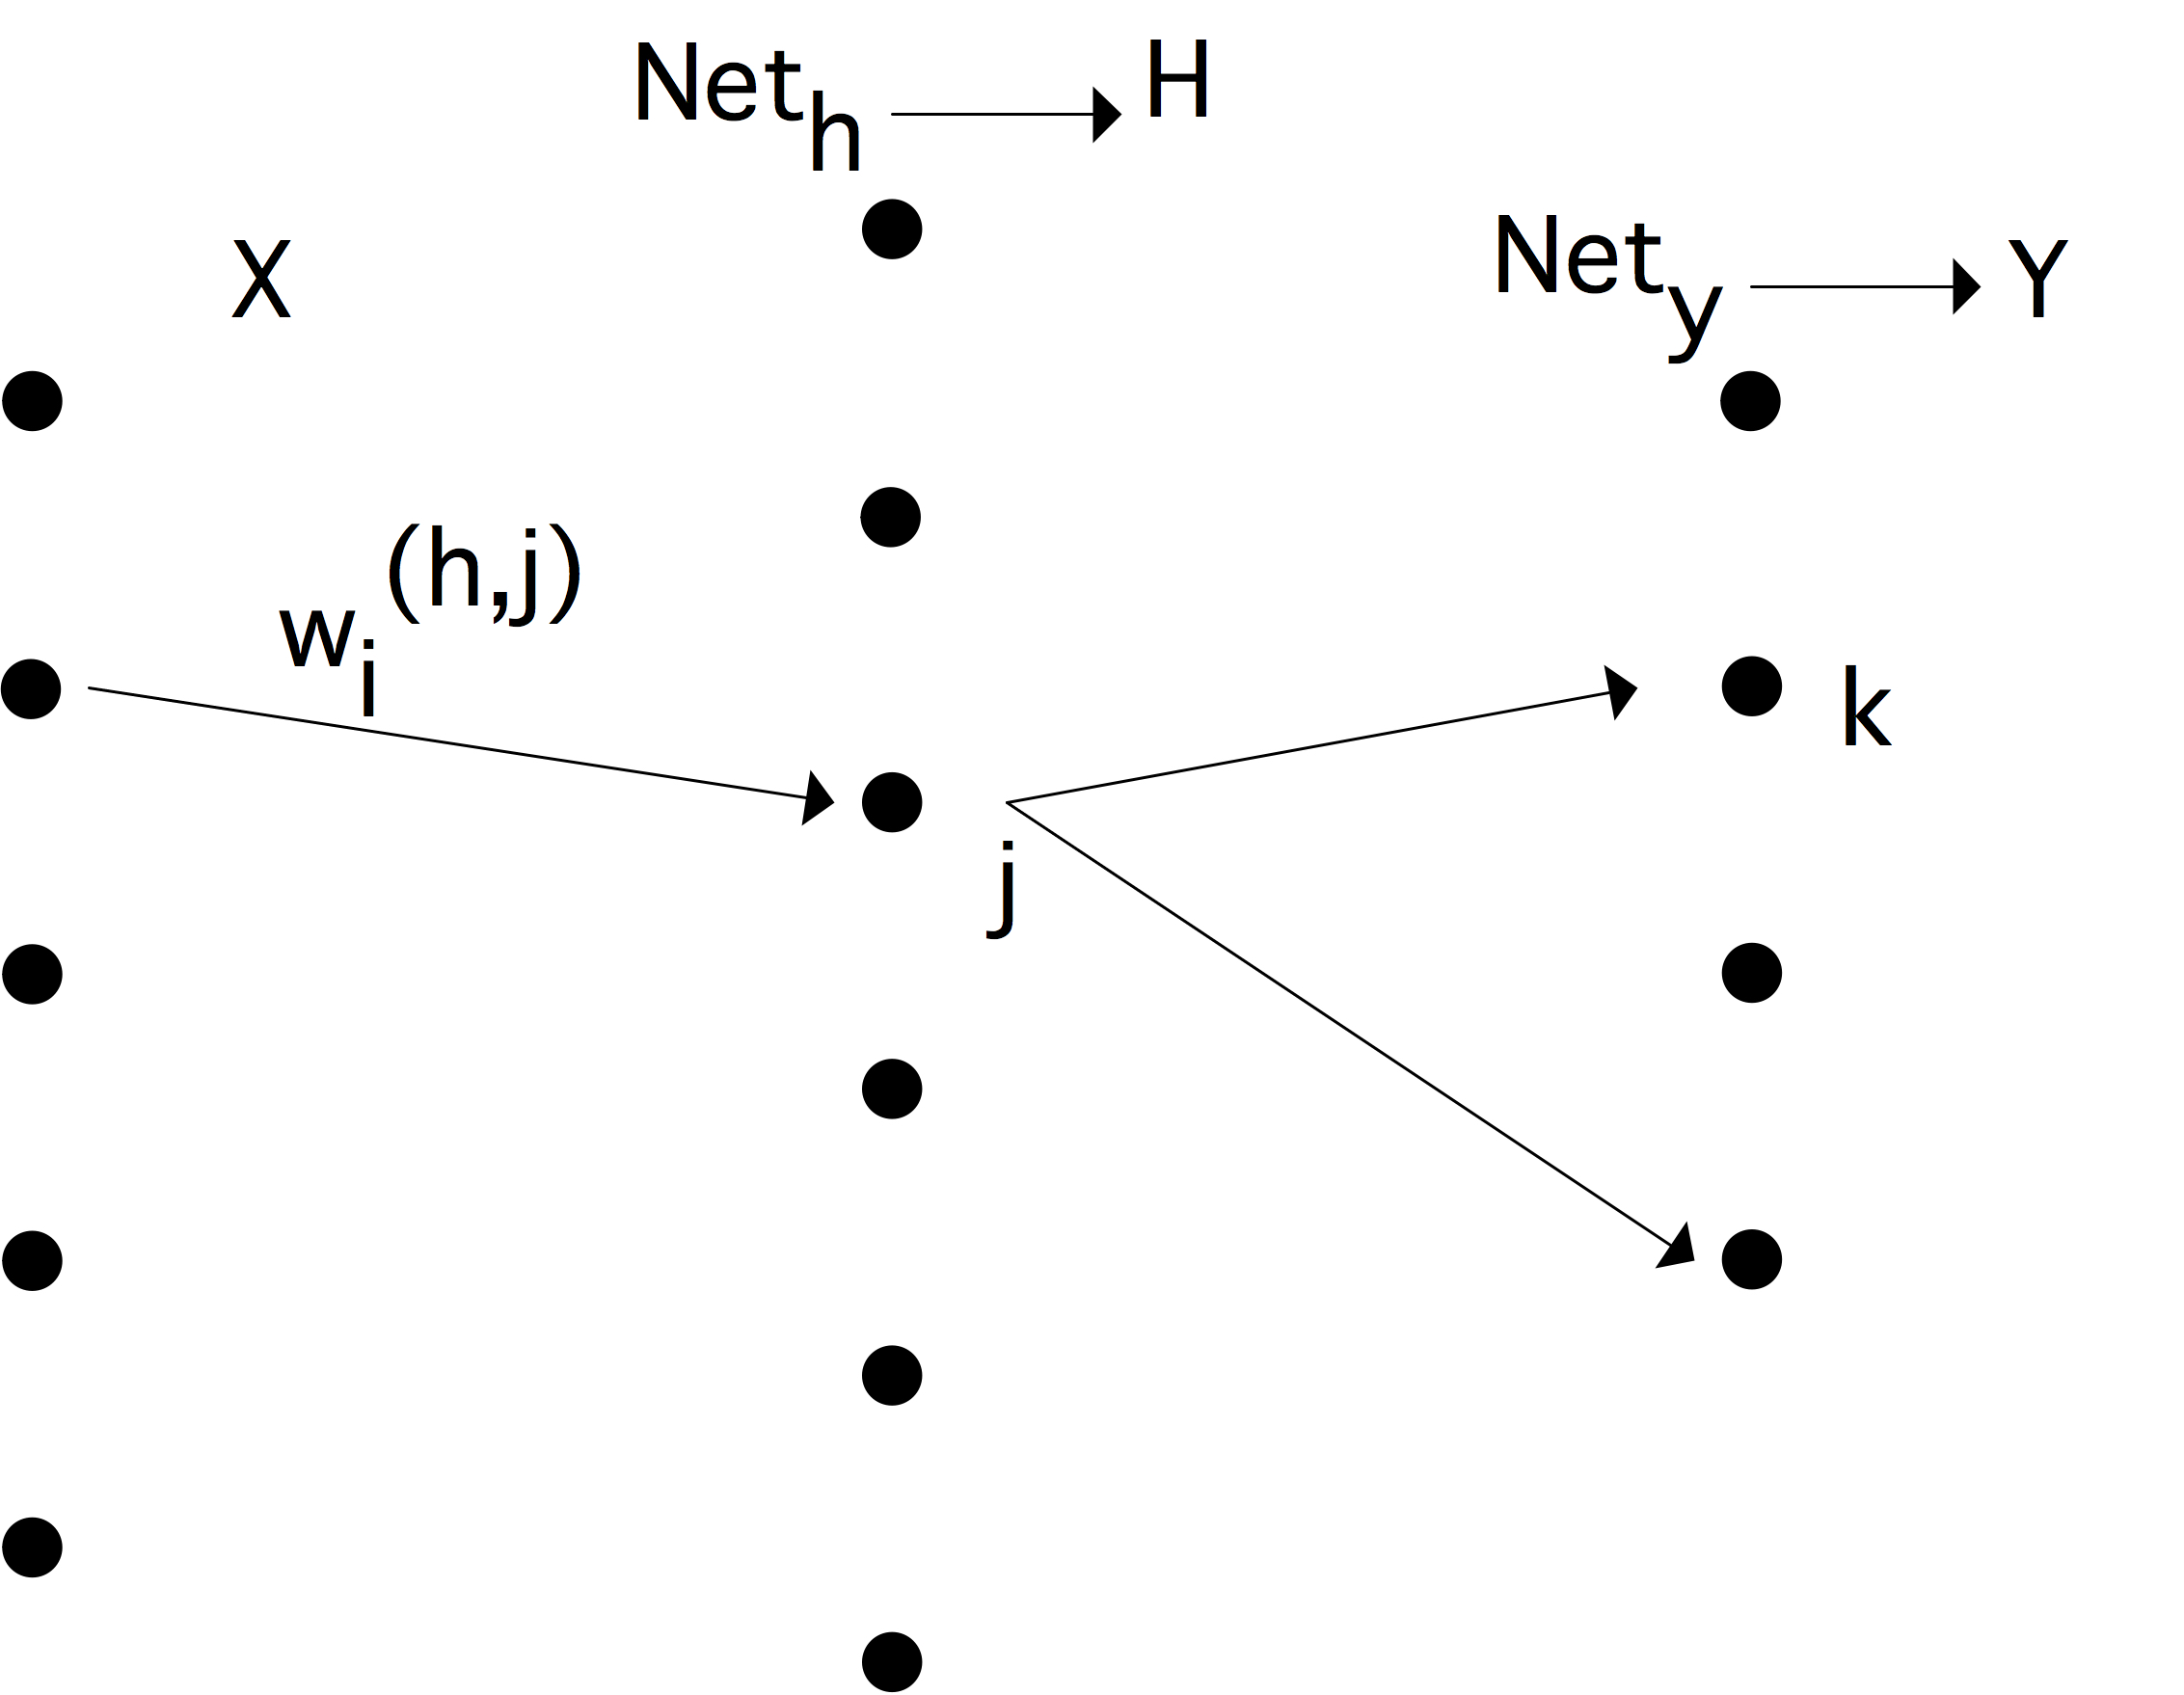
\includegraphics[scale=.12]{backpropagation-h}
  \caption{Back propagation, internal layer coefficients}
  \label{fig:backprop-h}
\end{figure}


\begin{lemma}
  \label{lemma:sigma-prime}
  \[ \sigma'(x) = \sigma(x)(1-\sigma(x)) \]
\end{lemma}
\begin{proof}
  \[
  \sigma'(x)=\frac{-1}{ (1+e^{-x})^2 }\cdot (-e^{-x})
  = \frac{e^{-x}}{ (1+e^{-x})^2 }
  = \frac{1}{ 1+e^{-x} } \frac{1+e^{-x}-1}{ 1+e^{-x} }
  \]
\end{proof}

For a worked out small example, see: \url{https://mattmazur.com/2015/03/17/a-step-by-step-backpropagation-example/}

\Level 0 {Computation}

GEMM in convolution kernels:
\url{https://petewarden.com/2015/04/20/why-gemm-is-at-the-heart-of-deep-learning/}
